\documentclass[border=0.2cm, 12pt]{standalone}
\usepackage{tikz}
\usepackage{amsmath, amssymb, amsfonts, mathtools}
\usepackage{color}
\begin{document}
  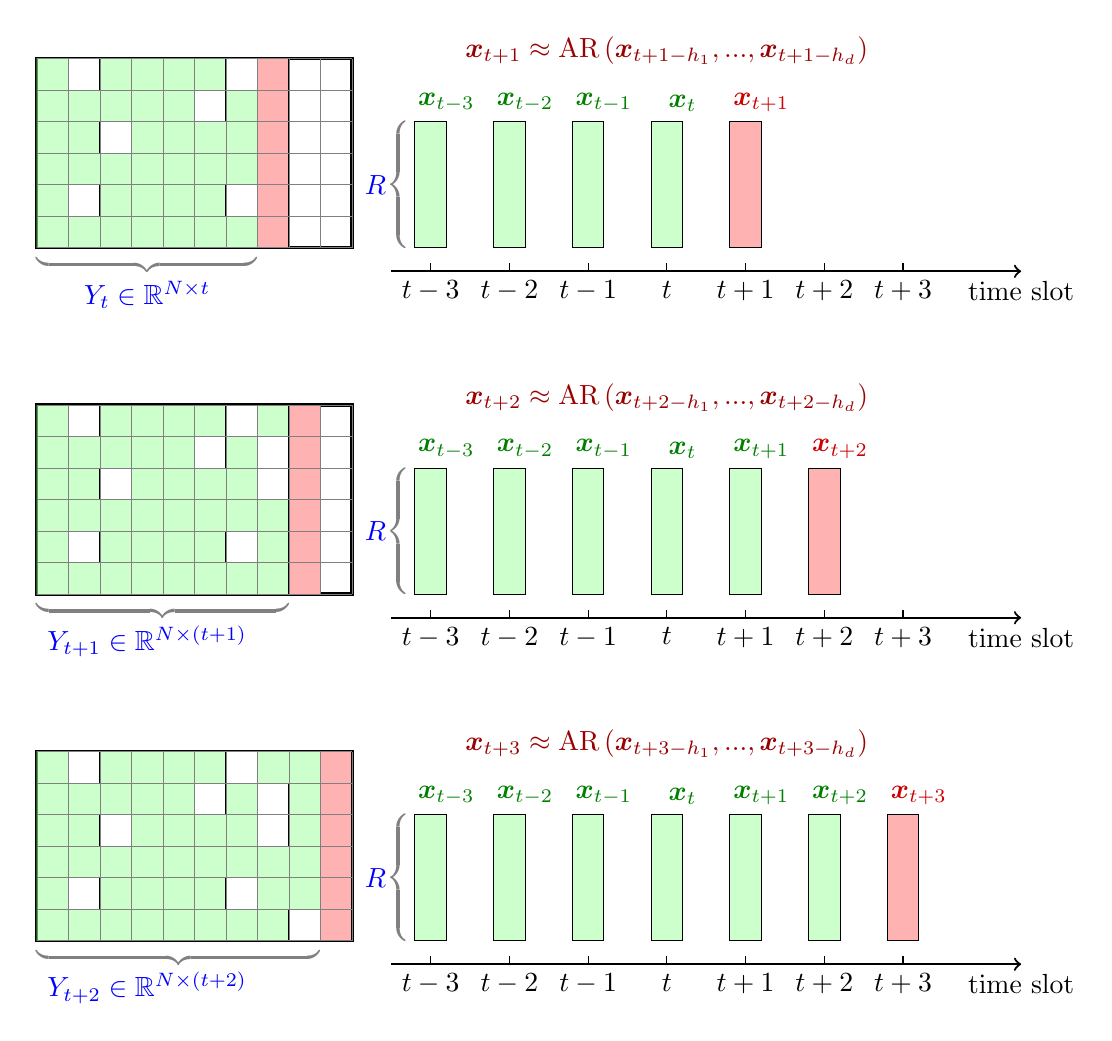
\begin{tikzpicture}[domain=0:4]
  % t step
    \draw [very thick] (0,0) rectangle (4,2.4);
    \filldraw [fill=green!20!white,draw=green!40!black] (0,0) rectangle (2.8,2.4);
    \filldraw [fill=red!30!white] (2.8,0) rectangle (3.2,2.4);
    \filldraw [fill=white] (0.4,0.4) rectangle (0.8,0.8);
    \filldraw [fill=white] (2.4,0.4) rectangle (2.8,0.8);
    \filldraw [fill=white] (0.8,1.2) rectangle (1.2,1.6);
    \filldraw [fill=white] (2.0,1.6) rectangle (2.4,2.0);
    \filldraw [fill=white] (0.4,2.0) rectangle (0.8,2.4);
    \filldraw [fill=white] (2.4,2.0) rectangle (2.8,2.4);
    \draw [step=0.4, very thin, color=gray] (0,0) grid (4,2.4);
    \draw (1.4,-0.6) node {{\color{blue}$Y_t\in\mathbb{R}^{N\times t}$}};
    \draw (1.4,-0.2) node[rotate = 0] {{\color{gray}$\underbrace{\hspace{2.8cm}}$}};

    \draw (5,-0.2) -- (5,-0.3) node[anchor=north,fill=white] {$t-3$};
    \draw (6,-0.2) -- (6,-0.3) node[anchor=north,fill=white] {$t-2$};
    \draw (7,-0.2) -- (7,-0.3) node[anchor=north,fill=white] {$t-1$};
    \draw (8,-0.2) -- (8,-0.3) node[anchor=north,fill=white] {$t$};
    \draw (9,-0.2) -- (9,-0.3) node[anchor=north,fill=white] {$t+1$};
    \draw (10,-0.2) -- (10,-0.3) node[anchor=north,fill=white] {$t+2$};
    \draw (11,-0.2) -- (11,-0.3) node[anchor=north,fill=white] {$t+3$};
    \draw [->, thick] (4.5,-0.3) -- (12.5,-0.3) node [below] {time slot};

    \filldraw [fill=green!20!white] (5-0.2,0) rectangle (5+0.2,1.6) node [above] {{\color{green!50!black}$\boldsymbol{x}_{t-3}$}};
    \filldraw [fill=green!20!white] (6-0.2,0) rectangle (6+0.2,1.6) node [above] {{\color{green!50!black}$\boldsymbol{x}_{t-2}$}};
    \filldraw [fill=green!20!white] (7-0.2,0) rectangle (7+0.2,1.6) node [above] {{\color{green!50!black}$\boldsymbol{x}_{t-1}$}};
    \filldraw [fill=green!20!white] (8-0.2,0) rectangle (8+0.2,1.6) node [above] {{\color{green!50!black}$\boldsymbol{x}_{t}$}};
    \filldraw [fill=red!30!white] (9-0.2,0) rectangle (9+0.2,1.6) node [above] {{\color{red!80!black}$\boldsymbol{x}_{t+1}$}};

    \draw (4.6,0.8) node[rotate = 270] {{\color{gray}$\underbrace{\hspace{1.6cm}}$}};
    \draw (4.3,0.8) node {{\color{blue}$R$}};
    \draw (8,2.5) node {{\color{red!60!black}$\boldsymbol{x}_{t+1}\approx\text{AR}\left(\boldsymbol{x}_{t+1-h_1},...,\boldsymbol{x}_{t+1-h_d}\right)$}};

  % t+1 step
    \draw [very thick] (0,0-4.4) rectangle (4,2.4-4.4);
    \filldraw [fill=green!20!white,draw=green!40!black] (0,0-4.4) rectangle (3.2,2.4-4.4);
    \filldraw [fill=red!30!white] (3.2,0-4.4) rectangle (3.6,2.4-4.4);
    \filldraw [fill=white] (0.4,0.4-4.4) rectangle (0.8,0.8-4.4);
    \filldraw [fill=white] (2.4,0.4-4.4) rectangle (2.8,0.8-4.4);
    \filldraw [fill=white] (0.8,1.2-4.4) rectangle (1.2,1.6-4.4);
    \filldraw [fill=white] (2.0,1.6-4.4) rectangle (2.4,2.0-4.4);
    \filldraw [fill=white] (0.4,2.0-4.4) rectangle (0.8,2.4-4.4);
    \filldraw [fill=white] (2.4,2.0-4.4) rectangle (2.8,2.4-4.4);
    \filldraw [fill=white] (2.8,1.2-4.4) rectangle (3.2,2.0-4.4);
    \draw [step=0.4, very thin, color=gray] (0,0-4.4) grid (4,2.4-4.4);
    \draw (1.4,-0.6-4.4) node {{\color{blue}$Y_{t+1}\in\mathbb{R}^{N\times (t+1)}$}};
    \draw (1.6,-0.2-4.4) node[rotate = 0] {{\color{gray}$\underbrace{\hspace{3.2cm}}$}};

    \draw (5,-0.2-4.4) -- (5,-0.3-4.4) node[anchor=north,fill=white] {$t-3$};
    \draw (6,-0.2-4.4) -- (6,-0.3-4.4) node[anchor=north,fill=white] {$t-2$};
    \draw (7,-0.2-4.4) -- (7,-0.3-4.4) node[anchor=north,fill=white] {$t-1$};
    \draw (8,-0.2-4.4) -- (8,-0.3-4.4) node[anchor=north,fill=white] {$t$};
    \draw (9,-0.2-4.4) -- (9,-0.3-4.4) node[anchor=north,fill=white] {$t+1$};
    \draw (10,-0.2-4.4) -- (10,-0.3-4.4) node[anchor=north,fill=white] {$t+2$};
    \draw (11,-0.2-4.4) -- (11,-0.3-4.4) node[anchor=north,fill=white] {$t+3$};
    \draw [->, thick] (4.5,-0.3-4.4) -- (12.5,-0.3-4.4) node [below] {time slot};

    \filldraw [fill=green!20!white] (5-0.2,0-4.4) rectangle (5+0.2,1.6-4.4) node [above] {{\color{green!50!black}$\boldsymbol{x}_{t-3}$}};
    \filldraw [fill=green!20!white] (6-0.2,0-4.4) rectangle (6+0.2,1.6-4.4) node [above] {{\color{green!50!black}$\boldsymbol{x}_{t-2}$}};
    \filldraw [fill=green!20!white] (7-0.2,0-4.4) rectangle (7+0.2,1.6-4.4) node [above] {{\color{green!50!black}$\boldsymbol{x}_{t-1}$}};
    \filldraw [fill=green!20!white] (8-0.2,0-4.4) rectangle (8+0.2,1.6-4.4) node [above] {{\color{green!50!black}$\boldsymbol{x}_{t}$}};
    \filldraw [fill=green!20!white] (9-0.2,0-4.4) rectangle (9+0.2,1.6-4.4) node [above] {{\color{green!50!black}$\boldsymbol{x}_{t+1}$}};
    \filldraw [fill=red!30!white] (10-0.2,0-4.4) rectangle (10+0.2,1.6-4.4) node [above] {{\color{red!80!black}$\boldsymbol{x}_{t+2}$}};

    \draw (4.6,0.8-4.4) node[rotate = 270] {{\color{gray}$\underbrace{\hspace{1.6cm}}$}};
    \draw (4.3,0.8-4.4) node {{\color{blue}$R$}};
    \draw (8,2.5-4.4) node {{\color{red!60!black}$\boldsymbol{x}_{t+2}\approx\text{AR}\left(\boldsymbol{x}_{t+2-h_1},...,\boldsymbol{x}_{t+2-h_d}\right)$}};

  % t+2 step
    \draw [very thick] (0,0-8.8) rectangle (4,2.4-8.8);
    \filldraw [fill=green!20!white,draw=green!40!black] (0,0-8.8) rectangle (3.6,2.4-8.8);
    \filldraw [fill=red!30!white] (3.6,0-8.8) rectangle (4.0,2.4-8.8);
    \filldraw [fill=white] (0.4,0.4-8.8) rectangle (0.8,0.8-8.8);
    \filldraw [fill=white] (2.4,0.4-8.8) rectangle (2.8,0.8-8.8);
    \filldraw [fill=white] (0.8,1.2-8.8) rectangle (1.2,1.6-8.8);
    \filldraw [fill=white] (2.0,1.6-8.8) rectangle (2.4,2.0-8.8);
    \filldraw [fill=white] (0.4,2.0-8.8) rectangle (0.8,2.4-8.8);
    \filldraw [fill=white] (2.4,2.0-8.8) rectangle (2.8,2.4-8.8);
    \filldraw [fill=white] (2.8,1.2-8.8) rectangle (3.2,2.0-8.8);
    \filldraw [fill=white] (3.2,0-8.8) rectangle (3.6,0.4-8.8);
    \draw [step=0.4, very thin, color=gray] (0,0-8.8) grid (4,2.4-8.8);
    \draw (1.4,-0.6-8.8) node {{\color{blue}$Y_{t+2}\in\mathbb{R}^{N\times (t+2)}$}};
    \draw (1.8,-0.2-8.8) node[rotate = 0] {{\color{gray}$\underbrace{\hspace{3.6cm}}$}};

    \draw (5,-0.2-8.8) -- (5,-0.3-8.8) node[anchor=north,fill=white] {$t-3$};
    \draw (6,-0.2-8.8) -- (6,-0.3-8.8) node[anchor=north,fill=white] {$t-2$};
    \draw (7,-0.2-8.8) -- (7,-0.3-8.8) node[anchor=north,fill=white] {$t-1$};
    \draw (8,-0.2-8.8) -- (8,-0.3-8.8) node[anchor=north,fill=white] {$t$};
    \draw (9,-0.2-8.8) -- (9,-0.3-8.8) node[anchor=north,fill=white] {$t+1$};
    \draw (10,-0.2-8.8) -- (10,-0.3-8.8) node[anchor=north,fill=white] {$t+2$};
    \draw (11,-0.2-8.8) -- (11,-0.3-8.8) node[anchor=north,fill=white] {$t+3$};
    \draw [->, thick] (4.5,-0.3-8.8) -- (12.5,-0.3-8.8) node [below] {time slot};

    \filldraw [fill=green!20!white] (5-0.2,0-8.8) rectangle (5+0.2,1.6-8.8) node [above] {{\color{green!50!black}$\boldsymbol{x}_{t-3}$}};
    \filldraw [fill=green!20!white] (6-0.2,0-8.8) rectangle (6+0.2,1.6-8.8) node [above] {{\color{green!50!black}$\boldsymbol{x}_{t-2}$}};
    \filldraw [fill=green!20!white] (7-0.2,0-8.8) rectangle (7+0.2,1.6-8.8) node [above] {{\color{green!50!black}$\boldsymbol{x}_{t-1}$}};
    \filldraw [fill=green!20!white] (8-0.2,0-8.8) rectangle (8+0.2,1.6-8.8) node [above] {{\color{green!50!black}$\boldsymbol{x}_{t}$}};
    \filldraw [fill=green!20!white] (9-0.2,0-8.8) rectangle (9+0.2,1.6-8.8) node [above] {{\color{green!50!black}$\boldsymbol{x}_{t+1}$}};
    \filldraw [fill=green!20!white] (10-0.2,0-8.8) rectangle (10+0.2,1.6-8.8) node [above] {{\color{green!50!black}$\boldsymbol{x}_{t+2}$}};
    \filldraw [fill=red!30!white] (11-0.2,0-8.8) rectangle (11+0.2,1.6-8.8) node [above] {{\color{red!80!black}$\boldsymbol{x}_{t+3}$}};

    \draw (4.6,0.8-8.8) node[rotate = 270] {{\color{gray}$\underbrace{\hspace{1.6cm}}$}};
    \draw (4.3,0.8-8.8) node {{\color{blue}$R$}};
    \draw (8,2.5-8.8) node {{\color{red!60!black}$\boldsymbol{x}_{t+3}\approx\text{AR}\left(\boldsymbol{x}_{t+3-h_1},...,\boldsymbol{x}_{t+3-h_d}\right)$}};
  \end{tikzpicture}
\end{document}
